\documentclass[a4paper, 14pt]{extarticle}
\usepackage{graphicx}
\usepackage[T2A]{fontenc}
\usepackage[utf8]{inputenc}
\usepackage[russian]{babel}
\usepackage{setspace,amsmath}
\usepackage[left=20mm, top=15mm, right=15mm, bottom=15mm, nohead, footskip=10mm]{geometry} % Настройки полей документа

\graphicspath{ {./images/} }

\makeatletter
\def\@seccntformat#1{
  \expandafter\ifx\csname c@#1\endcsname\c@section\else
  \csname the#1\endcsname\quad
  \fi}
\makeatother

\makeatletter
\newcommand{\verbatimfont}[1]{\renewcommand{\verbatim@font}{\ttfamily#1}}
\makeatother

\begin{document} % Начало документа

% Начало титульного листа
\begin{center}
    \normalsize{\textbf{МИНИСТЕРСТВО ОБРАЗОВАНИЯ РЕСПУБЛИКИ БЕЛАРУСЬ}}\\
    \hfill \break
    \normalsize{\textbf{БЕЛОРУССКИЙ ГОСУДАРСТВЕННЫЙ УНИВЕРСИТЕТ}}\\
    \hfill \break
    \small{\textbf{ФАКУЛЬТЕТ ПРИКЛАДНОЙ МАТЕМАТИКИ И ИНФОРМАТИКИ}}\\
    \hfill \break
    \large{Кафедра математического моделирования и анализа данных}\\
    \vspace{40mm}
    \normalsize{Дипломная работа}\\
    \hfill \break
    \normalsize{Криптография на основе функций хэширования:\\ подписи без состояния}\\
    \hfill \break
\end{center}

\begin{flushright}
    \vspace{20mm}
    Болтач Антон Юрьевич\\
    Студент 4 курса 9 группы\\
    Научный руководитель\\
    С. В. Агиевич\\
\end{flushright}

\vfill
\begin{center}
    Минск, 2020 г.
\end{center}
\thispagestyle{empty} % Выключаем отображение номера для этой страницы
    
% Конец титульного листа

\newpage

% Содержание
\tableofcontents
\newpage

% Введение
% Концепции Hash-based crypto
\section{Введение}
Цифровые подписи широко используются в Интернете, в частности, для аутентификации, проверки целостности и отказа от авторства. Алгоритмы цифровой подписи, наиболее часто используемые на практике - RSA, DSA и ECDSA, - основаны на допущениях твердости о задачах теории чисел, а именно факторизации составного целого числа и вычислении дискретных логарифмов. В 1994 году Питер Шор показал, что эти теоретические проблемы с числами могут стать решаемыми при наличии квантовых вычислений. Квантовые компьютеры могут решить их за полиномиальное время, ставя под угрозу безопасность схем цифровой подписи, используемых сегодня. Хотя квантовые компьютеры еще не доступны, их развитие происходит быстрыми темпами и поэтому представляет собой реальную угрозу в течение следующих десятилетий. К счастью, постквантовая криптография предоставляет множество квантовостойких альтернатив классическим схемам цифровой подписи. Подписи на основе хэша или подписи Меркля, как они также известны, являются одной из наиболее многообещающих из этих альтернатив.
\subsection{Почему Hash-Based Signatures?}
Есть много причин использовать схемы подписи на основе хэша и предпочитать их другим альтернативам. Хотя в самой ранней схеме подписи отсутствуют практические требования к производительности и пространству, современные схемы на основе хэшей, такие как XMSS, достаточно быстры, при небольшом размере. Также требования безопасности являются убедительными. Использование такой схемы подписи всегда требует хэш-функции. В то время как другие схемы подписи полагаются на дополнительные предположения о неразрешимости для генерации подписи, для решения на основе хэша требуется только безопасная хэш-функция. Некоторые схемы, основанные на хэше, даже уменьшают потребность в хэш-функции, устойчивой к столкновениям, до той, которая должна выдерживать атаки только на второе изображение. В качестве примера известны практические атаки средствами защиты от столкновений функции MD5, но мы до сих пор не знаем о виртуальных атаках на второе изображение.
\newpage

% Одноразовые подписи
\section{Одноразовые подписи(OTS)}
Одноразовые подписи ($OTS$) называются одноразовыми, поскольку сопутствующие сокращения безопасности гарантируют безопасность только при атаках с одним сообщением. Однако это не означает, что эффективные атаки возможны при атаках с двумя сообщениями. Особенно в контексте основанных на хэшировании $OTS$ (которые являются основными строительными блоками последних предложений по стандартизации) это приводит к вопросу о том, приводит ли случайное повторное использование одноразовой пары ключей к немедленной потере безопасности. Проанализируем безопасность наиболее известных $OTS$ на основе функций хэширования: $WOTS$, $WOTS^{+}$ при различных видах атак с двумя сообщениями. Интересно, что оказывается, что схемы все еще безопасны при двух атаках сообщений, асимптотически.
\subsection{Одноразовая подпись Винтерница($WOTS$)}
$WOTS$ использует функцию сохранения длины $F : \{0, 1\}^{n} \rightarrow \{0, 1\}^{n}$. Она параметризуется длиной сообщения $m$ и параметром $Winternitz$, $w \in N$, $w > 1$, который определяет компромисс между временем и памятью. Эти два параметра используются для вычисления
\[ l_{1} = \Bigg \lceil \frac{m}{log(w)} \Bigg \rceil, l_{2} = \Bigg \lfloor \frac{log(l_{1}(w - 1))}{log(w)} \Bigg \rfloor + 1, l = l_{1} + l_{2}. \]
Схема использует $w - 1$ итераций $F$ на случайном входе. Мы определяем их как
\[ F^{a}(x) = F(F^{a - 1}(x)) \]
и $F^{0}(x) = x$.
\newline

\textbf{Теперь опишем три этапа алгоритма подписи:}

\begin{itemize}
    \item \textbf{Алгоритм генерации ключей $(kg(1^{n}))$:}
    
    На входе параметр безопасности $1^{n}$ алгоритм генерации ключей выбирает $l$ ($n$-битовых блоков) равномерно, случайным образом. Личный ключ $sk = (sk_{1}, ..., sk_{l})$ состоит из этих $l$ блоков случайных битовых строк. Открытый ключ проверки $pk$ вычисляется как
    \[ pk = (pk_{1}, ..., pk_{l}) = (F^{w - 1}(sk_{1}), ..., F^{w - 1}(sk_{l})) \]

    \item \textbf{Алгоритм подписи$(sign(1^{n}, M^{*}, sk))$:}

    На входе параметр безопасности $1^{n}$, сообщение $M^{*}$ длины $m$ и личного ключа подписи $sk$, алгоритм подписи сначала вычисляет базовое $w$ представление $M^{*}: M^{*} = (M^{*}_{1}, ..., M^{*}_{l_{1}}), M^{*}_{i} \in \{0, ..., w - 1\}$. Далее он вычисляет контрольную сумму
    \[ C = \sum^{l_{1}}_{i = 1}(w - 1 - M^{*}_{i}) \]

    и вычисляет его базовое $w$ представление $C = (C_{1}, ..., C_{l_2})$. Длина базового $w$ представления $C$ не более $l_{2}$, так как $C \leq l_{1}(w - 1)$. Мы задаем $B = (B_{1}, ..., B_{l}) = M^{*} || C$. Подпись вычисляется как
    \[ \sigma = (\sigma_{1}, ..., \sigma_{l}) = (F^{B_1}(sk_{1}), ..., F^{B_l}(sk_{l})) \]

    \item \textbf{Алгоритм проверки $(vf(1^{n}, M^{*}, \sigma, pk))$:}

    На входе параметр безопасности $1^{n}$, сообщение $M^{*}$ длины $m$, подпись $\sigma$ и открытый ключ проверки $pk$, алгоритм проверки сначала вычисляет $B_{i}$, $ 1 \leq i \leq l$, как описано выше. Затем он выполняет следующее сравнение:
    \[ pk = (pk_{1}, ..., pk_{l}) \stackrel{?}= (F^{w - 1 - B_{1}}(\sigma_{1}), ..., (F^{w - 1 - B_{l}}(\sigma_{l})) \]
    Если сравнение выполняется, оно возвращает $true$ или $false$ в противном случае.
\end{itemize}

\subsection{Дополненная подпись Винтерница($WOTS^{+}$)}
Теперь опишем $WOTS^{+}$. Как и все варианты $W\-OTS$, $W\-OTS^{+}$ параметризуется параметром безопасности $n \in N$, длиной сообщения $m$ и параметром $w \in N$, $w > 1$, который определяет компромисс между временем и памятью. Последние два параметра используются для вычисления
\[ l_{1} = \Bigg \lceil \frac{m}{log(w)} \Bigg \rceil, l_{2} = \Bigg \lfloor \frac{log(l_{1}(w - 1))}{log(w)} \Bigg \rfloor + 1, l = l_{1} + l_{2}. \]

Кроме того, $W\-OTS^{+}$ использует семейство функций $F_{n} : \{f_{k} : \{0, 1\}^{n} \rightarrow \{0, 1\}^{n}|k \in K_{n}\}$ с ключевым пространством $K_{n}$. Можно предположить как о криптографическом семействе хэш-функций, которое не сжимается. Используя $F_{n}$, мы определяем следующую функцию.

$c^{i}_{k}(x, r):$ На входе значения $x \in \{0, 1\}^{n}$, счетчика итераций $i \in N$, ключа $k \in K$ и элементы случайности $r = (r_{1}, ..., r_{j}) \in \{0, 1\}^{n \times j}$ при $j \geq i$, функция работает следующим образом:

\begin{itemize}
    \item В случае $i = 0$, $c^{i}_{k}(x, r)$ возвращает $x(c^{0}_{k}(x, r) = x)$.
    \item Для $i > 0$ мы определяем $c^{i}_{k}(x, r)$ рекурсивно как
    \[ c^{i}_{k}(x, r) = f_{k}(c^{i - 1}_{k}(x, r) \oplus r_{i}) ,\]
\end{itemize}

То есть в каждом раунде функция сначала принимает побитовый $xor$ промежуточного значения и битовую маску $r$, затем оценивает $f_{k}$ на результат. Мы пишем $r_{a,b}$ для подмножества $r_{a}, ..., r_{b}$ как $r$. В случае $b < a$ мы определяем $r_{a,b}$ как пустую строку. Будем считать, что параметры $m$, $w$ и семейство функций $F_{n}$ общеизвестны.

\textbf{Теперь опишем три этапа алгоритма подписи $W\-OTS^{+}$:}

\begin{itemize}
    \item \textbf{Алгоритм генерации ключа $(Kg(1^n))$:}

    При вводе параметра безопасности $n$ унарно, алгоритм генерации ключа выбирает $l + w - 1$ $n$-бит строки равномерно случайным образом. Личный ключ $sk = (sk_{1}, ..., sk_{l})$ состоит из первых $l$ случайных битовых строк. Оставшиеся $w - 1$ бит строки используются в качестве элементов случайности $r = (r_{1}, ..., r_{w - 1})$ для $c$. Далее, $Kg$ выбирает функцию ключа $k \stackrel{\$}\leftarrow K$ равномерно случайным образом. Открытый ключ проверки $pk$ вычисляется как
    \[ pk = (pk_{0}, pk_{1}, ..., pk_{l}) = ((r, k),c^{w - 1}_{k}(sk_{1},r), ..., c^{w - 1}_{k}(sk_{l}, r)). \]

    \item \textbf{Алгоритм подписи $(Sign(M, sk, r))$:}

    На входе $m$ битного сообщения $M$, личного ключа подписи $sk$ и элементов случайности $r$, алгоритм подписи сначала вычисляет базовое $w$ представление $M: M = (M_{1} . . . M_{l_{1}} )$, $M_{i} \in \{0, ..., w - 1\}$. Поэтому $M$ рассматривается как двоичное представление натурального числа $x$, а затем вычисляется $w$ бинарное представление $x$. Далее вычисляем контрольную сумму
    \[ C = \sum^{l_{1}}_{i = 1}(w - 1 - M_{i}) \]
    и его базовое $w$ представление $C = (C_{1}, ..., C_{l_{2}})$. Длина базового $w$ представления $C$ не более $l_{2}$, так как $C \leq l_{1}(w - 1)$. Мы задаем $B = (b_{1}, ..., b_{l}) = M || C$, конкатенация базовых $w$ представлений $M$ и $C$. Подпись вычисляется как
    \[ \sigma = (\sigma_{1}, ..., \sigma_{l}) = (c^{b_{1}}_{k}(sk_{1},r), ..., c^{b_{l}}_{k}(sk_{l},r)). \]

    Обратите внимание, что контрольная сумма гарантирует, что с учетом $b_{i}, 0 < i \leq l$, соответствующего одному сообщению, $b^{*}_{i}$ соответствующий любому другому сообщению включает по крайней мере один $b^{*}_{i} < b_{i}$.

    \item \textbf{Алгоритм проверки $(Vf(1^n, M, \sigma, pk))$:}

    На входе сообщение $M$ двоичной длины $m$, подпись $\sigma$ и открытый ключ $pk$. Алгоритм проверки сначала вычисляет $b_{i}, 1 \leq i \leq l$, как описано выше. Затем он выполняет следующее сравнение:
    \[ pk = (pk_{0}, pk_{1}, ..., pk_{l}) \stackrel{?}{=} ((r,k),c^{w - 1 - b_{1}}_{k}(\sigma_{1}, r_{b_{1} + 1, w - 1}, ..., c^{w - 1 - b_{l}}_{k}(\sigma_{l}, r_{b_{l} + 1, w - 1}))\]

    Если сравнение выполняется, оно возвращает $true$ или $false$ в противном случае.
\end{itemize}

Время выполнения всех трех алгоритмов ограничено $l$ и $w$ оценками $f_{k}$. Размер подписи и личного ключа составляет $|\sigma| = |sk| = l*n$ бит. Размер открытого ключа равен $(l + w - 1)n + |k|$ бит, где $|k|$ обозначает количество бит, необходимых для представления любого элемента $K$.
\subsubsection{Обоснование стойкости($WOTS^{+}$)}
В этом разделе мы анализируем безопасность $WOTS^{+}$.

Определение($\epsilon$-доступность обнаружения подделки). $\epsilon$-доступность обнаружения подделки($\epsilon$-$FDA$) для одноразового $WOTS^{+}$ S определяется следующим экспериментом.

Эксперимент $Exp^{F D A}_{S,n}(A)$:

\hspace{10mm} $(sk, pk) \leftarrow S.Kg(1^n)$

\hspace{10mm} $(M^{*}, \sigma^{*}) \leftarrow A^{Sign(sk,\cdot)}$

Пусть $(M, \sigma)$ будьте парой запрос-ответ $Sign(sk,\cdot)$.

Вернём 1, если $S.Sign(sk, M^{*}) \rightarrow \sigma^{*}, S.Verify(pk, \sigma^{*}, M^{*}) \rightarrow 1, M^{*} \neq M$.

Тогда схема $WOTS^{*}$ $S$ имеет $\epsilon-FDA$, если нет противника $A$, который преуспевает с вероятностью $\geq \epsilon$.

Построим схему $(n, \delta, L, \nu)-W\-OTS^{+}$ следующим образом.

Введем параметр $\nu \in \{1, 2, ...\}$ определение длины блоков, в которых сообщение разбивается во время алгоритма подписи, где мы предполагаем, что $L$ кратно $\nu$. 

Введем следующие вспомогательные значения:
\[w := 2^{\nu}, l_{1} := \lceil L/\nu \rceil, l_{2} := \lfloor log_{2}(l_{1}(w - 1))/\nu \rfloor + 1, l := l_{1} + l_{2}\]

Затем рассмотрим семейство односторонних функций:
\[ f^{(i)}_{r} : \{0,1\}^{n+\delta(w - i)} \rightarrow \{0,1\}^{n+\delta(w - i - 1)} \]

где $i \in \{1, ..., w - 1\}$ и параметр $r$ принадлежит некоторой области $D$. Мы предполагаем, что $f^{(i)}_{r}$ удовлетворяет случайному предположению оракула для равномерно случайно выбранного $r$ из $D$. Использование этого параметра может соответствовать $XOR$ некоторого семейства хэш-функций со случайной битовой маской.

Затем мы вводим функцию $F^{(i)}_{r}$, которую мы определяем рекурсивно следующим образом:
\[F^{(0)}_{r}(x) = x, F^{(i)}_{r}(x) = f^{(i)}_{r}(F^{(i - 1)}_{r}(x)), i \in \{1, ..., w - 1\}.\]
\newpage % FIXME: see pdf result
\textbf{Алгоритм схемы $(n, \delta, L, \nu)-W\-OTS^{+}$ делится на три этапа:}
конкатенация
\begin{itemize}
    \item \textbf{Алгоритм генерации пары ключей:}

    Сперва алгоритм генерирует личный ключ в следующем виде:
    \[sk := (r, sk_{1}, sk_{2}, ..., sk_{l}), sk_{i} \stackrel{\$}{\leftarrow} \{0, 1\}^{n+\delta(w - 1)}, r \stackrel{\$}{\leftarrow} D\]
    (Рис. \ref{fig:wots1}). Затем открытый ключ, состоящий из случайного параметра $r$ и результаты функции, используемой для $sk_{i}$ следующим образом:
    \[ pk := (r, pk_{1}, pk_{2}, ..., pk_{l}), pk_{i} := F^{w - 1}_{r}(sk_{i})\]

    \begin{figure}[h]
        \centering
        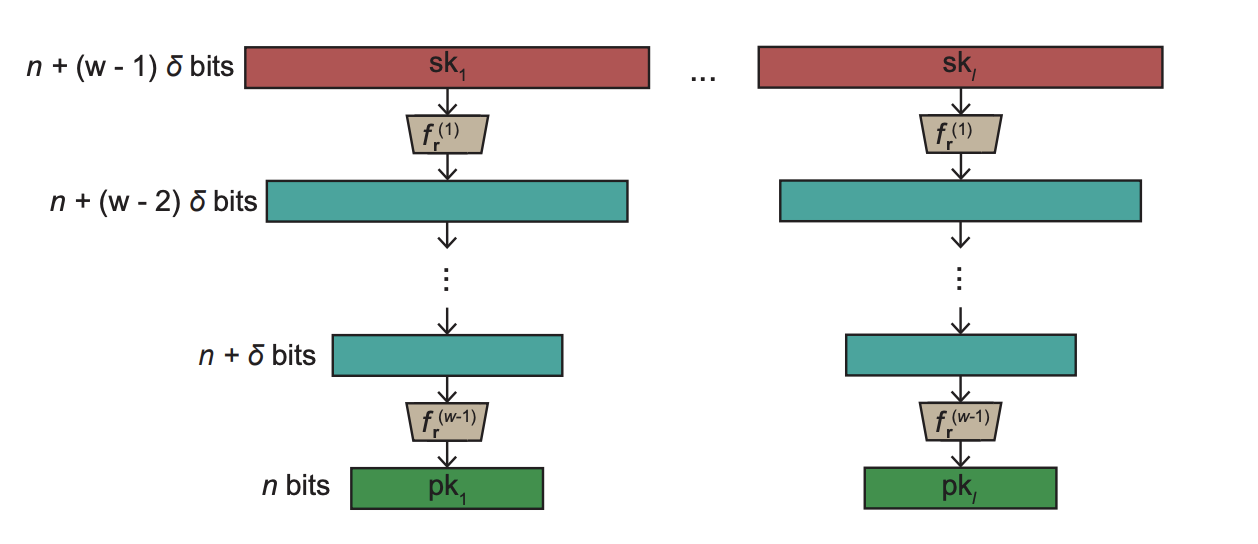
\includegraphics[scale=0.78]{WOTS+_1.png}
        \caption{Основной принцип построения открытого ключа в схеме $(n, \delta, L, \nu)-WOTS^{+}$ }
        \label{fig:wots1}
    \end{figure}

    \item \textbf{Алгоритм подписи сообщения:}

    Сперва алгоритм вычисляет базовое $w$ представление $M$, разбивая его на $\nu$-битные блоки $(M = (m_{1}, ..., m_{l_{1}})$, где $m_{i} \in \{0, ..., w - 1\})$. Затем алгоритм вычисляет контрольную сумму
    \[ C := \sum^{l_{1}}_{i = 1}(w - 1 - m_{i}) \]
    и его базовое $w$ представление $C = (c_{1}, ..., c_{l_{2}})$. Определим расширенную строку $B = (b_{1}, ..., b_{l}) := M||C$ как конкатенация частей сообщения и контрольной суммы. Наконец, подпись генерируется следующим образом:
    \[ \sigma = (\sigma_{1}, ..., \sigma_{l}), \sigma_{i} := F^{(b_{i})}_{r}(sk_{i}). \]

    \item \textbf{Алгоритм проверки подписи:}

    Идея алгоритма состоит в том, чтобы восстановить открытый ключ из заданной подписи $\sigma$ и затем проверить, совпадает ли он с исходным открытым ключом $pk$. Во-первых, алгоритм вычисляет базовую $w$ строку $B = (B_{1}, ..., B_{l})$ таким же образом, как и в алгоритме подписи (см. выше). Затем для каждой части подписи $\sigma_{i}$ алгоритм вычисляет оставшуюся часть цепочки следующим образом:
    \[pk^{check}_{i} := f^{(w - 1)}_{r} \circ ... \circ f^{(b_{i}+1)}_{r}(\sigma_{i}),\]
    где $\circ$ композиция функций. Если $pk^{check}_{i} = pk_{i}$ для всех $i \in \{1, ..., l\}$, затем алгоритм выводит $\nu := 1$, иначе $\nu := 0$.
\end{itemize}

Основной результат по свойству FDA схемы $(n, \delta, L, \nu)-W\-OTS^{+}$ можно сформулировать следующим образом:

Теорема. $(n, \delta, L, \nu)-W\-OTS^{+}$ схема имеет свойство $\epsilon-FDA$ с $\epsilon < 5.22 \times 2^{-\delta}$.

Доказательство. Рассмотрим сценарий успешного CMA на схеме $(n, \delta, L, \nu)-W\-OTS^{+}$, в которой противник сначала выступает в роли законного пользователя с открытым ключом $pk = (r, pk_{1}, ..., pk_{l})$, чтобы предоставить ему подпись $\sigma = (\sigma_{1}, ..., \sigma_{l})$ для некоторого сообщения $M$, а затем генерирует действительную подпись $\sigma^{*} = (\sigma^{*}_{1}, ..., \sigma^{*}_{l})$ для какого-то сообщения $M^{*} \neq M$. Пусть $(m_{1}, ..., m_{l})$ и $(m^{*}_{1}, ..., m^{*}_{l})$ будут $w$ представления $M$ и $M^{*}$ соответственно. Рассмотрим расширенные $w$ строки $B = (b^{0}_{1}, ..., b^{0}_{l})$ и $B^{*} = (b^{*}_{1}, ..., b^{*}_{l})$, которые генерируется путем добавления частей контрольной суммы. Легко заметить, что для любого отличного $M$ и $M^{*}$ существует по крайней мере одна позиция $j \in \{1, ..., l\}$ такая, что $b^{*}_{j} < b_{j}$. Действительно, даже если для всех позиций $i \in \{1, ..., l_{1}\}$ случилось, что $m^{*}_{i} > m_{i}$, из определения контрольной суммы следует, что существует позиция $j \in \{l_{1} + 1, ..., l_{2}\}$ в части суммы такие, что $b^{*}_{j} < b_{j}$.

Поскольку $\sigma^{*}$ допустима. Подпись для $M^{*}$:
\[f^{(w - 1)}_{r} \circ ... \circ f^{(b^{*}_{j} + 1)}_{r}(\sigma^{*}_{j}) = pk_{j}.\]
Можно заметить, что событие подделки будет обнаружено, если $j$-ая часть подписи законного пользователя $M^{*}$ отличается от фальшивого (см. также Рис. \ref{fig:wots2}), так что:
\[\stackrel{\sim}{\sigma^{*}_{j}} := F^{(b^{*}_{j})}_{r}(sk_{j}) \neq \sigma^{*}_{j}.\]

\begin{figure}[h]
    \centering
    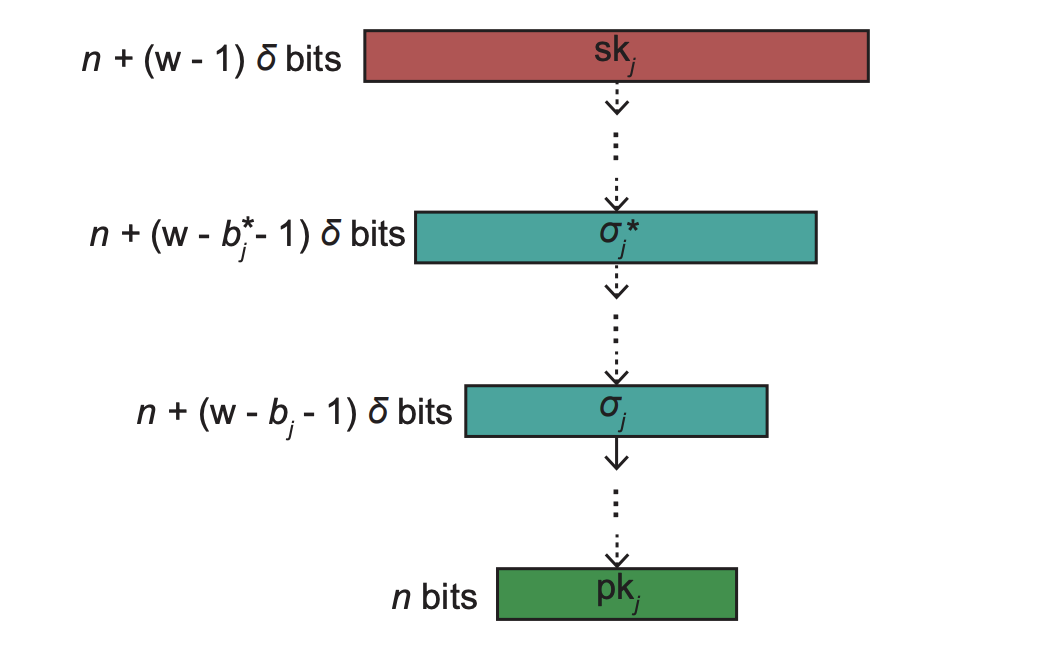
\includegraphics[scale=0.65]{WOTS+_2.png}
    \caption{Иллюстрация принципа построения доказательство подделки типа 2 для схемы $(n, \delta, L, \nu)-WOTS^{+}$. }
    \label{fig:wots2}
\end{figure}

\newpage

\textbf{Рассмотрим два возможных случая:}

\begin{itemize}
    \item Во-первых, условие из теоремы выполняется, но справедливо следующее соотношение:

    \[f^{(b_{j})}_{r} \circ ... \circ f^{(b^{*}_{j}+1)}_{r}(\sigma^{*}_{j}) \neq \sigma_{j}.\]
    В этом случае мы получаем $\stackrel{\sim}{\sigma^{*}_{j}} \neq \sigma^{*}_{j}$ с единичной вероятностью так как
    \[\sigma_{j} = f^{(b_{j})}_{r} \circ ... \circ f^{(b^{*}_{j}+1)}_{r}(\stackrel{\sim}{\sigma^{*}_{j}}) \neq f^{(b_{j})}_{r} \circ ... \circ f^{(b^{*}_{j}+1)}_{r}(\sigma^{*}_{j}).\]

    \item Во втором случае мы имеем следующее тождество:

    \[f^{(b_{j})}_{r} \circ ... \circ f^{(b^{*}_{j}+1)}_{r}(\sigma^{*}_{j}) = \sigma_{j},\]
    что автоматически подразумевает выполнение условия теоремы. Рассмотрим функцию
    \[F := f^{(b_{j})}_{r} \circ ... \circ f^{(b^{*}_{j}+1)}_{r} : \{0, 1\}^{n^{*} + \delta \Delta} \rightarrow \{0,1\}^{n^{*}},\]
    где $\Delta := b^{0}_{j} - b^{*}_{j} \geq 1$ и $n^{*} := n + \delta(w - b^{*}_{j} - 1)$. Эта функция удовлетворяет случайным предположениям оракула, так как каждый из $\{f^{(k)}_{r}\}^{b_{j}}_{k=b^{*}_{j}}$. Следовательно мы имеем вероятность того, что противник получит $\sigma^{*}_{j} = \stackrel{\sim}{\sigma^{*}_{j}}$ с ограничением $\epsilon < 5.22 \times 2^{-\delta \Delta} \leq 5.22 \times 2^{-\delta}$. Что и требовалось доказать.
\end{itemize}
\newpage

% Деревья Меркля
\section{Деревья Меркля(MSS)}
Первый способ создать схему многократной подписи из схемы одноразовой подписи - использовать конструкцию, предложенную Мерклом в 1989 году. Учитывая целые числа $n$, $h$ и хэш-функцию $H$ : $\{0, 1\}^{2n} \rightarrow \{0, 1\}^{n}$, так называемое Дерево Меркля представляет собой двоичное дерево высоты $h$, узлы которого помечены значением $x \in \{0, 1\}^{n}$, таким образом, что значение каждого внутреннего узла вычисляется как $x = H(y||z)$, где $y$ и $z$ - значения левых и правых дочерних элементов.

Корневое значение $r$ может быть сначала отправлено для последующей аутентификации любого из $2^{h}$ листового значения $v_{1}, ..., v_{2^h}$. Действительно, чтобы проверить, что значение $v$ находится в листовом индексе $i$, нужны $v$, $i$ и путь аутентификации $i$. Этот путь аутентификации содержит братьев и сестер всех узлов на пути между листом $i$ и корнем (значения $h$). Это позволяет рекурсивно вычислять значения внутренних узлов вплоть до корня и сравнивать результат с $r$.

Эта конструкция позволяет превратить схему одноразовой подписи в схему многократной подписи следующим образом. Учитывая $2^h$ экземпляров OTS, подписывающий создает дерево Меркля, каждое листовое значение которого являются открытым ключом экземпляра OTS. Общий открытый ключ - это корневое значение. $i$-я подпись содержит подпись, сгенерированную $i$-м экземпляром OTS, а также путь аутентификации $i$.

Следовательно, открытый ключ содержит только $n$ битов, по сравнению с подходом $2^h$ OTS открытых ключей. Однако время генерации ключа экспоненциально в $h$, потому что на этом этапе необходимо вычислить полное дерево Меркля. Например, $h$ = 20 возможно, но может быть недостаточно для всех подписывающих. Кроме того, подписывающий должен отслеживать индексы $i$, которые уже были использованы, поэтому схема является $stateful$.
\newpage

% Многоразовые подписи
\section{Многоразовые подписи(MTS)}
В то время как одноразовые подписи обеспечивают удовлетворительную криптографическую безопасность для подписания и проверки транзакций, для них характерен существенный недостаток - их можно использовать безопасно только один раз. Поэтому существуют схемы подписи для включения более чем одной действительной одноразовой подписи, что позволяет сформировать предварительно столько подписей, сколько будет пар ключей одноразовых подписей. Логичным путем достижения этого является построение двоичного хэш-дерева, известного как дерево Меркля.
\subsection{HORS}
$HORS$ - это несколькоразовая схема подписи. Пусть $f$ - односторонняя функция, а $H$ - хэш-функция, которая выводит случайный размер подмножества $\{1,2,...,t\}$, где $k$ и $t$ - параметры, влияющие на безопасность с помощью $k < t$. Ключ подписи - это случайный кортеж $(s_1,...,s_t)$, а открытым ключом является $(f(s_{1}),..., f(s_{t}))$. 
Теперь, чтобы подписать $m$ сообщение, вычислить набор $S = H(m)$ и выходной $\{s_{i} : i \in S\}$. Чтобы проверить, примените $f$ к каждому элементу подписи и проверьте, соответствует ли он открытому ключу. Каждая подпись раскрывает $k$ элементов личного ключа, поэтому в зависимости от выбора $k$ и $t$ несколько сообщений могут быть подписаны до того, как безопасность будет нарушена. Это было использовано в качестве строительного блока в $SPHINCS$, который представляет собой схему подписи на основе хэша без состояния, которая позволяет подписывать неограниченные количество сообщений.

\begin{figure}[h]
    \centering
    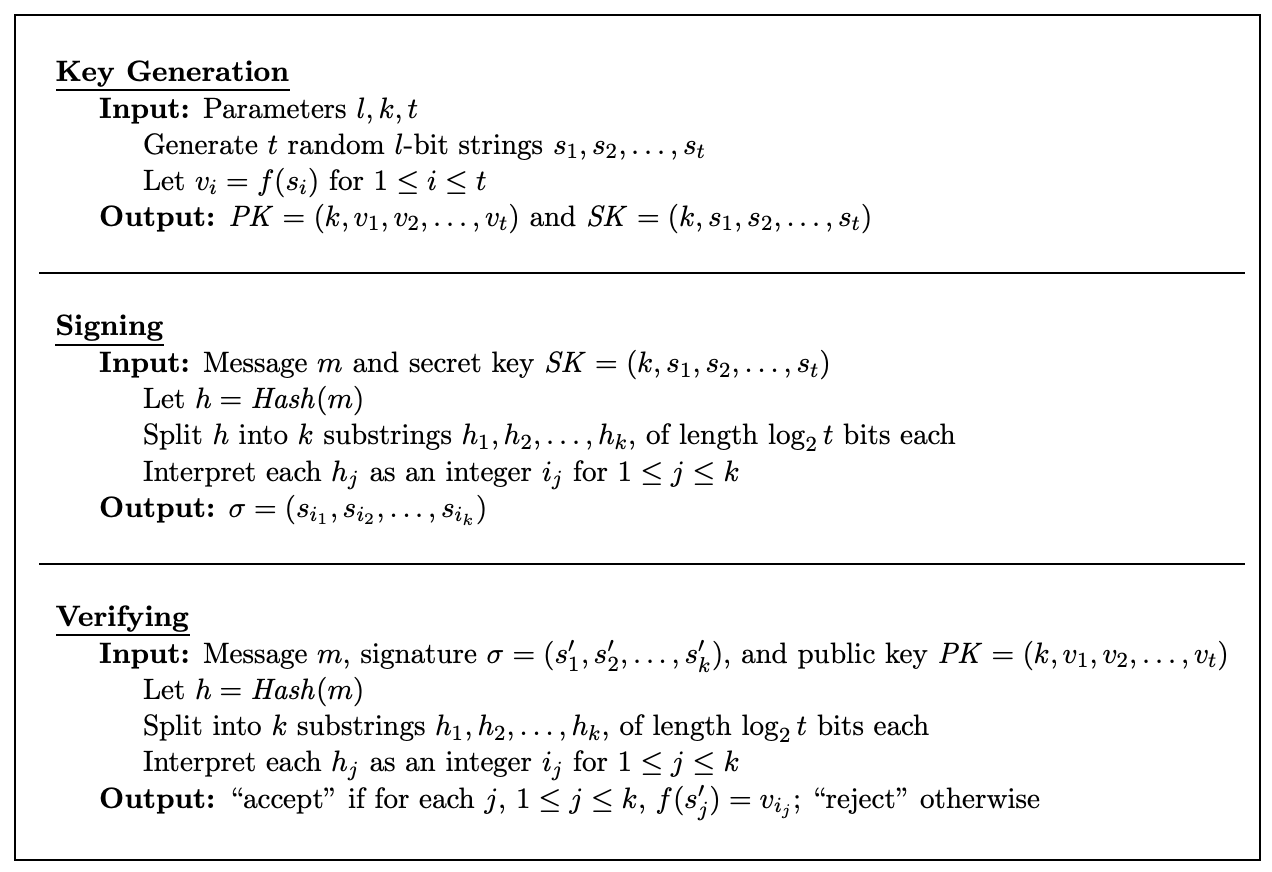
\includegraphics[scale=0.62]{HORS.png}
    \caption{Схема подписи HORS}
    \label{fig:hors}
\end{figure}

\subsection{PORS}
Начнём с того, что $PORS$, более безопасный вариант $HORS$. Как мы видели, современные схемы с несколькими временными подписями основаны на хэше для получения случайного подмножества. Тем не менее, $HORS$ была изучена лишь частично, так как Рейзин и Рейзин(отец и сын) рассматривали только неадаптивные атаки. В частности, $HORS$ подвержен адаптивным атакам, которые усугубляются простотой $HORS$: возьмите выход хэш-функции и разделите его на блоки, чтобы получить набор индексов. Действительно, ничто не мешает некоторым из этих индексов сталкиваться, уменьшая размер полученного подмножества и уменьшая безопасность. Несмотря на то, что $HORS$ показывает себя как простая и быстрая подпись по сравнению с более сложными методами получения случайных подмножеств гарантированного размера, его скорость не критична в сложных схемах, таких как $SPHINCS$, для которых голоса и деревья Меркля доминируют в вычислительных затратах. Поэтому рассмотрим новую конструкцию, для получения случайного подмножества, которое мы называем $PORS$. Вместо того, чтобы использовать хэш-функцию, мы выполняем запрос к ней, пока мы не получим подмножество различных индексов (Рис. \ref{fig:pors}). Вычислительные издержки эквивалентны нескольким дополнительным вычислениям хэша для значительного повышения безопасности. В случае $SPHINCS$ заметим, что противники имеют полный контроль над выбранным листом в гипердереве. Вместо этого мы предлагаем создать этот листовой индекс, что ещё больше повысит уровень безопасности. Этот увеличенный запас прочности позволяет уменьшить высоту гипердерева на 2 слоя, экономя 4616 байт.

\begin{figure}[h]
    \centering
    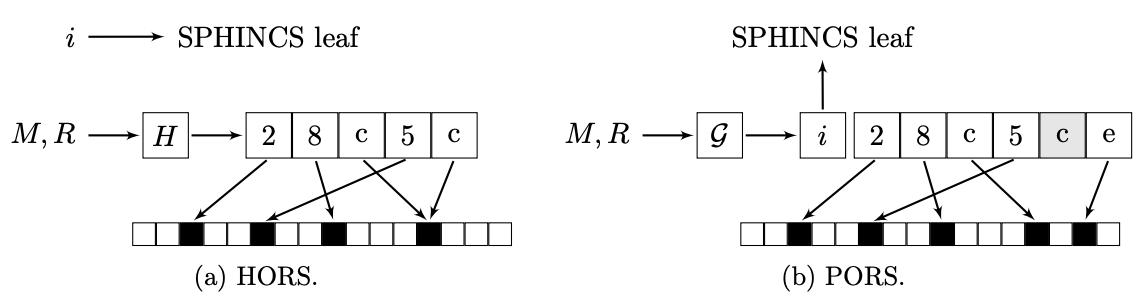
\includegraphics[scale=0.86]{PORS.png}
    \caption{Сравнение HORS и PORS}
    \label{fig:pors}
\end{figure}
\newpage

% Подписи без состояния
\section{Подписи без состояния}
\subsection{SPHINCS}
Представим основные идеи $SPHINCS$, описав его как комбинацию четырех типов деревьев. Ниже перечислены четыре типа деревьев (см. Рис. \ref{fig:SPHINCS}):

\begin{figure}[h]
    \centering
    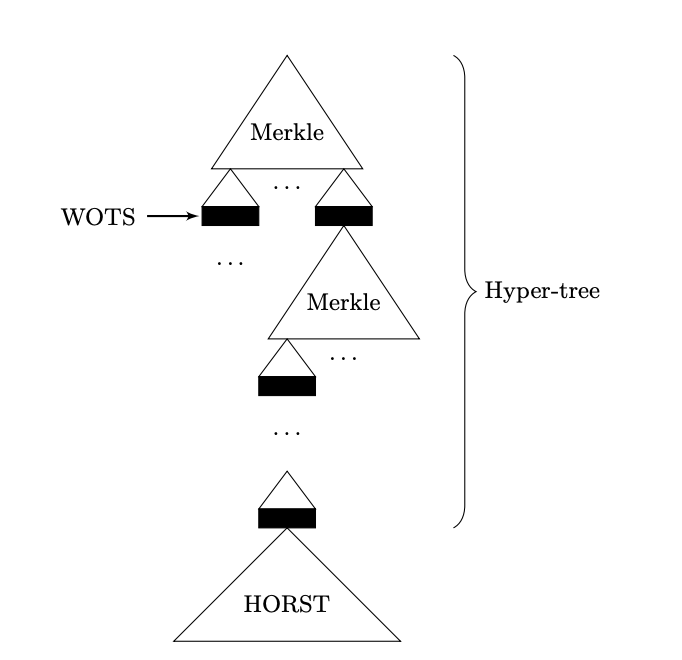
\includegraphics[scale=0.85]{SPHINCS.png}
    \caption{Пример $SPHINCS$. Гипердерево состоит из $d$ слоев дерева Меркля и соединены $WOTS$. Внизу дерево $HORS$(или $HORST$) соединяется с подписанным сообщением.}
    \label{fig:SPHINCS}
\end{figure}

\begin{enumerate}
    \item Главное Гипердерево, высотой $h$ (60 в $SPHINCS-256$). Корень этого дерева является частью открытого ключа. Листья этого дерева экземпляры $HORST$. Это Гипердерево делится на $d$ слоев($d$ = 12 в $SPHINCS-256$).
    \item Поддеревья, которые являются деревьями Меркля высоты $h/d$ (60/12 = 5 в $SPHINCS-256$). Листья этих деревьев являются корнями деревьев; указанные корни являются сжатыми открытыми ключами экземпляров $WOTS$, которые соединяются с деревом на следующем уровне.
    \item Открытый ключ $WOTS$ это деревья сжатия, которые являются \newline L-деревьями, высоты $\lceil log_{2}l \rceil$.Листья этого дерева являются компонентами $WOTS$ открытого ключа (67 значений по 256 бит каждое в $SPHINCS-256$). Связанный экземпляр $WOTS$ подписывает корень дерева на следующем уровне.
    \item В нижней части гипердерева, открытый ключ $HORST$ - деревья сжатия это деревья Меркля высоты $\tau = log_{2}t$, где $t$ номер элементов открытого ключа $HORST$($2^{16}$ в $SPHINCS-256$).
\end{enumerate}

\textbf{Подписание в $SPHINCS$ работает следующим образом:}

\begin{enumerate}
    \item Извлекается листовой индекс из сообщения и личного ключа. Этот индекс определяет один из экземпляров $2^{h} HORST$ (относительно основного гипердерева), который будет использоваться для подписи сообщения.
    \item Создайте экземпляр $HORST$, который является производным от личного ключа и конечного индекса, и подпишите сообщение этим экземпляром $HORST$. Подпись $HORST$ включает $k$ ключей и их соответствующие пути аутентификации и является частью подписи $SPHINCS$. Итого получаем сжатый в дереве $HORST$ открытый ключ $p$.
    \item Для каждого слоя гипердерева подпишите открытый ключ $p$(полученный из нижнего слоя), используя правильный экземпляр $WOTS$(полученный из листового индекса); добавьте эту подпись $WOTS$ и связанный с ней путь аутентификации к подписи $SPHINCS$. Вычислите путь аутентификации этого экземпляра $WOTS$ в поддереве. Добавьте этот путь к подписи $SPHINCS$ и $p$-корень поддерева.
\end{enumerate}

\subsection{Gravity-SPHINCS}
$Gravity-SPHINCS$ наследуют некоторые параметры от $SPHINCS$ (длина хэша, глубина $WOTS$ и др.), а так же имеет новые. В приведенном ниже списке $h$ обозначает высоту поддеревьев(в отличие от высоты основного дерева в $SPHINCS$), а $B_{n} = \{0,1\}^{n}$ обозначает набор $n$-битовых строк.
\newline

\textbf{Параметры являются следующими:}

\begin{itemize}
    \item Хэш-выход длина бита $n$, положительное целое число.
    \item Глубина $WOTS$ $w$, степень 2-ки такой, что $w \geq 2$ и $log_{2}w$ делит $n$.
    \item Размер множества $PORS$ $t$, положительное, степень двойки.
    \item Размер подмножества $PORS$ $k$, положительное целое такое, что $k \leq t$.
    \item Высота дерева Меркля $h$, положительное целое.
    \item Количество внутренних деревьев Меркля $d$, неотрицательное целое.
    \item Высота кэша $c$, неотрицательное целое.
    \item Высота $b$, неотрицательное целое.
    \item Пространство сообщения $M$, обычно подмножество битовых строк $\{0,1\}^{*}$.
\end{itemize}

\newpage

\textbf{Из этих параметров получены:}

\begin{itemize}
    \item Размер $WOTS$ $l = \mu + \lfloor log_{2}(\mu(w - 1))/log_{2}w \rfloor + 1$, где $\mu = n/log_{2}w$.
    \item Множество $PORS$, $T = \{0, ..., t - 1\}$.
    \item Адресное пространство $A = \{0, ..., d\} \times \{0, ..., 2^{c + dh} - 1\} \times \{0, ..., max(l,t) - 1\}$.
    \item Пространство открытых ключей $PK = B_{n}$.
    \item Пространство личных ключей $SK = B^{2}_{n}$.
    \item Пространство подписи $SG = B_{n} \times B^{k}_{n} \times B^{\leq k(log_{2}t - \lfloor log_{2}k \rfloor)}_{n} \times (B^{l}_{n} \times B^{h}_{n})^{d} \times B^{c}_{n}$.
    \item $SG_{B} = B^{b}_{n} \times \{0, ..., 2^{b} - 1\} \times SG$
    \item Размер открытого ключа $n$ бит.
    \item Размер личного ключа, $2n$ бит.
    \item Максимальный размер подписи
    \[sigsz = (1 + k +k(log_{2}t - \lfloor log_{2}k \rfloor) + d(l + h) + c)n\]
\end{itemize}

Алгоритм подписи $Sign$ одного сообщения и проверка $Verify$ в $Gravity-SPHINCS$ очень похожа на $SPHINCS$.
\newline

\textbf{Опишем три этапа алгоритма подписи $Gravity-SPHINCS$:}

\begin{itemize}
    \item \textbf{Алгоритм генерации ключей:}

    $KG$ получает на вход $2n$ случайных бит и на выходе получаем личный ключ $sk \in B^{2}_{n}$, и открытый ключ $pk \in B_{n}$.

    \begin{enumerate}
        \item Генерация личного ключа из $2n$ случайных бит:
        \[sk = (seed, salt) \stackrel{\$}{\leftarrow} B^{2}_{n}\]

        \item Для $0 \leq i < 2^{c+h}$ генерируется $Winternitz$ открытый ключ:
        \[x_{i} \leftarrow WOTS, \text{используя } genpk(seed, make-addr(0, i))\]

        \item Генерация открытого ключа:
        \[pk \leftarrow Merkle, \text{используя } root_{c+h}(x_{0}, ..., x_{2^{c+h} - 1})\]
    \end{enumerate}
    \newpage
    \item \textbf{Алгоритм подписи:}

    $S$ на вход принимает хэш $m \in B_{n}$ и личный ключ $sk = (seed, salt)$, и на выходе получаем подпись.

    \begin{enumerate}
        \item Вычисляем $s \leftarrow H(salt, m)$.

        \item Вычисляем гипердерева индекс и случайное подмножество как
        \[j, (x_{1}, ..., x_{k}) \leftarrow PORS(s, m)\]

        \item Вычисляем $PORST$ подпись и открытый ключ:
        \[(\sigma_{d}, oct, p), \text{используя } sign(seed, make-addr(d, j), x_{1}, ..., x_{k})\]

        \item Для $i \in \{d - 1, ..., 0\}$ выполняется:
        
        \begin{enumerate}
            \item Вычисляем $WOTS$ подпись:
            \[\sigma_{i} \leftarrow WOTS, \text{используя } sign(seed, make-addr(i,j),p)\]

            \item Вычисляем $p \leftarrow WOTS, \text{используя } extractpk(p, \sigma_{i})$.

            \item $j^{*} \leftarrow \lfloor j / 2^{h} \rfloor$.

            \item Для $u \in \{0, ..., 2^{h} - 1\}$ вычислим $WOTS$ открытый ключ:
            \[p_{u} \leftarrow WOTS, \text{используя } genpk(seed, make-addr(i, 2^{h}, j^{*} + u))\]

            \item Вычислим Меркля аутентификацию:
            \[A_{i} \leftarrow Merkle, \text{используя } auth_{h}(p_{0}, ..., p_{2^{h} - 1}, j - 2^{h}j^{*})\]

            \item $j \leftarrow j^{*}$.
        \end{enumerate}

        \item Для $0 \leq u < 2^{c+h}$ вычислим $WOTS$ открытый ключ:
        \[p_{u} \leftarrow WOTS, \text{используя } genpk(seed, make-addr(0, u))\]

        \item Вычислим Меркля аутентификацию:
        \[(a_{1}, ..., a_{h+c}) \leftarrow Merkle, \text{используя } auth_{h+c}(p_{0}, ..., p_{2^{h+c} - 1}, 2^{h}j)\]

        \item $A_{c} \leftarrow (a_{h+1}, ..., a_{h+c})$.

        \item Получаем подпись $(s, \sigma_{d}, oct, \sigma_{d - 1}, A_{d - 1}, ..., \sigma_{0}, A_{0}, A_{c})$.
    \end{enumerate}

    \item \textbf{Алгоритм проверки подписи:}

    $V$ получает на вход хэш $m \in B_{n}$, открытый ключ $pk \in B_{n}$ и подпись
    \[(s, \sigma_{d}, oct, \sigma_{d - 1}, A_{d - 1}, ..., \sigma_{0}, A_{0}, A_{c})\]
    и проверяет это следующим образом:

    \begin{enumerate}
        \item Вычислим индекс гипердерева и случайное подмножество
        \[j, (x_{1}, ..., x_{k}) \leftarrow PORS(s,m)\]

        \item Вычислим открытый ключ $PORST$,
        \[p \leftarrow PORST, \text{используя } extractpk(x_{1}, ..., x_{k}, \sigma_{d}, oct).\]

        \item Если $p = \perp$, затем прерываем и возвращаем 0.

        \item Для $i \in \{d - 1, ..., 0\}$ выполняем следующее:

        \begin{enumerate}
            \item Вычислим открытый ключ $WOTS$:
            \[p \leftarrow WOTS, \text{используя } extractpk(p, \sigma_{i})\]
            \item $j^{*} \leftarrow \lfloor j/2^{h} \rfloor$.
            \item Вычислим корень дерева Меркля:
            \[p \leftarrow Merkle, \text{используя } extract_{h}(p, j - 2^{h}j^{*}, A_{i})\]
            \item $j \leftarrow j^{*}$.
        \end{enumerate}

        \item Вычислим корень дерева Меркля:
        \[p \leftarrow Merkle, \text{используя } extract_{c}(p, j, A_{c})\]

        \item В результате 1, если $p = pk$ и 0 в ином случае.
    \end{enumerate}
\end{itemize}

\subsection{SPHINCS+}
$SPHINCS^{+}$ использует псевдослучайную функцию $PRF$ для генерации ключей, $PRF : \{0, 1\}^{n} \times \{0, 1\}^{256} \rightarrow \{0, 1\}^{n}$, и псевдослучайную функцию $PRF_{msg}$ для генерации случайного сжатия сообщения: $PRF_{msg} : \{0, 1\}^{n} \times \{0, 1\}^{n} \times \{0, 1\}^{*} \rightarrow \{0, 1\}^{n}$. Для сжатия подписываемого сообщения мы используем дополнительную хэш-функцию $H_{msg}$, которая может обрабатывать сообщения произвольной длины:
\[H_{msg} : \{0, 1\}^{n} \times \{0, 1\}^{n} \times \{0, 1\}^{n} \times \{0, 1\}^{*} \rightarrow \{0, 1\}^{m}\]

\textbf{$SPHINCS^{+}$ Личный и открытый ключ:}

\begin{itemize}
    \item Открытый ключ состоит из двух $n$-битных значений: корневого узла из трех верхних в гипердереве и случайного открытого начального значения $PK$.
    \item Личный ключ состоит еще из двух $n$-битных случайных: $SK$, чтобы генерировать $WOTS^{+}$ и $FORS$ личные ключи, и $SK.prf$, используемый ниже для случайного дайджеста сообщений.
\end{itemize}

\textbf{$SPHINCS^{+}$ Подпись сообщения.}

Как не удивительно, что подпись состоит из $FORS$ подписи для дайджеста сообщения, $WOTS^{+}$ подпись соответствующих открытых ключей $FORS$, ряда каналов аутентификации для подтверждения того, что $WOTS^{+}$ является открытым ключом. Чтобы проверить эту цепочку путей и подписей, проверка итеративно восстанавливает открытые ключи и корневые узлы до тех пор, пока не будет достигнут корневой узел в верхней части гипердерева $SPHINCS^{+}$. 
\newline

\textbf{Два момента еще не были рассмотрены:}

\begin{itemize}
    \item Вычисление дайджеста сообщения.
    \item Выбор листа.
\end{itemize}

Здесь $SPHINCS^{+}$ отличается от оригинальных $SPHINCS$ тонкими, но важными деталями.

Во-первых, мы псевдо случайным образом генерируем случайные числа $R$, основанные на сообщении и $SK.prf$. $R$ может быть дополнительно сконструирован недетерминированным путем добавления дополнительной случайности $OptRand$. Это может противодействовать атакам бокового канала, которые полагаются на сбор нескольких следов для одного и того же вычисления. Обратите внимание, что установка этого значения в нулевую строку (или использование значения с низкой энтропией) не оказывает отрицательного влияния на псевдослучайность $R$. Формально, мы полагем, что $R = PRF(SK.prf, OptRand, M)$. $R$ часть подписи. Используя $R$, мы затем получаем индекс конечного узла, который должен использоваться, а также получаем дайджест сообщения $(MD||idx) = H_{msg}(R, PK, PK.root, M)$.

В отличие от $SPHINCS$, этот метод выбора индекса является публично проверяемым, не позволяя злоумышленнику свободно выбирать кажущийся случайным индекс и комбинировать его с сообщением по своему выбору. Критически важно, что это противодействует многоцелевым атакам на схему подписи $FTS$. Поскольку индекс теперь может быть вычислен верификатором, он больше не включается в подпись.
\newpage

% Сравнение Stateful && Stateless
\section{Stateful vs Stateless}
Схемы с сохранением состояния имеют дерево Меркля с количеством одноразовых подписей внизу. Каждая разовая подпись может быть использована один раз, следовательно, подписывающий должен отслеживать, какие из них он использовал. То есть, когда он использует одноразовую подпись для подписи сообщения, он должен обновить свое состояние.

Схемы без состояния имеют большое дерево, но внизу у них есть несколько подписей времени. Каждая такая небольшая временная подпись может подписать несколько сообщений. Таким образом, когда подписывается сообщение, подписывающий выбирает случайную подпись с небольшим количеством времени, использует ее для подписи сообщения, а затем подтверждает ее подлинность через деревья Меркля вплоть до корня, который является открытым ключом. Поскольку мы используем несколько раз подпись, мы не против, если мы иногда выбираем одну и ту же подпись несколько раз. Схема подписи $FTS$ может справиться с этим. И, поскольку нам не нужно обновлять какое-либо состояние при генерации подписи, это считается «без сохранения состояния».
\newpage

% Введение в Bitshares
\section{Bitshares}
В 2013 году под авторством $Daniel$ $Larimer$ был опубликована статья с упоминанием $Bitshares$. Идея протокола $Bitshares$ состоит в создании платформы, с помощью которой можно было бы торговать разными активами и валютами в децентрализованной среде. Статья обсуждалась на научных конференциях по блокчейну. Так $Daniel$ $Larimer$ познакомился с еще одним активным криптовалютным деятелем по имени $Charles$ $Hoskinson$, который помог проработать бизнес-план и привлечь инвестиции.

\subsection{Назначение платформы Bitshares}
Протокол реализует децентрализованную биржу, где этими цифровыми активами можно торговать. При проектировании учетной системы и механизма достижения консенсуса разработчики сделали большой упор на пропускную способность. Как результат, $Bitshares$ позиционирует себя как децентрализованная альтернатива учетной системе $Visa$. В то время как $Visa$ заявляет, что может обрабатывать пару десятков тысяч транзакций в секунду, $Bitshares$ говорит о способности обрабатывать сто тысяч транзакций в секунду, причем децентрализованным образом, с открытой базой данных и возможностью аудита.

\subsection{Достижение консенсуса на основе DPoS}
Правила работы протокола $DPoS$ предполагают, что все пользователи могут принимать участие в достижении консенсуса, выбирая валидаторов посредством голосования. В процессе голосования вес голоса пользователя определяется его балансом в базовой валюте. Формирование блоков выполняется подмножеством избранных валидаторов. В рамках протокола $Bitshares$ валидатор называется $witness$.

\subsection{Модель транзакций}
Детальнее остановимся на модели транзакций в $Bitshares$. Т.к. основная работа заключалась в замене подписи транзакций в данной платформе на квантовостойкие. (см. Рис. \ref{fig:Bitshares_trx_model}).

\begin{figure}[h]
    \centering
    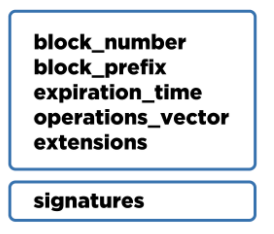
\includegraphics[scale=0.5]{Bitshares_trx_model.png}
    \caption{Модель транзакции в $Bitshares$}
    \label{fig:Bitshares_trx_model}
\end{figure}

На схеме видно, что тело транзакции состоит из пяти основных полей. Первые два поля транзакции необходимы для того, чтобы привязать ее к определенному блоку. Это нужно, чтобы определить цепочку блоков, в которую эта транзакция может быть добавлена, поскольку по правилам протокола транзакция не может быть подтверждена в той цепочке, к которой не привязана. Поле $expiration\_time$ задает время, до которого транзакция может быть добавлена в блок. Если она не была подтверждена до наступления этого времени, то она считается невалидной и уже не может быть включена в блокчейн.

Поле $operations\_vector$ является особенным. Эта особенность состоит в том, что в него можно поместить много разных операций. Операция — это еще один ключевой объект в протоколе $Bitshares$. Назовем несколько самых популярных типов операций: $transfer$ (перевод), $account\_update$ (обновление аккаунта), $asset\_issue$ (выпуск токена) Каждая операция имеет свой формат и необходимые параметры. Например, операция $transfer$ требует указания аккаунта отправителя, типа актива, суммы перевода и аккаунта получателя. Сами операции независимы друг от друга, но могут быть выполнены только вместе, если транзакция будет принята. То есть мы можем сделать несколько переводов средств между аккаунтами и выпустить все эти переводы одной транзакцией.

Поле $extensions$ сделано для обратной совместимости, чтобы текущая версия программного обеспечения могла обрабатывать транзакции новой версии, где могут быть добавлены дополнительные поля. Конечно же, старое ПО не будет знать, как правильно верифицировать дополнительные поля новых транзакций, но хотя бы сможет корректно обрабатывать транзакции согласно старым правилам.

Это формат неподписанной транзакции. Для того чтобы транзакцию правильно подписать, нужно проанализировать все операции из $operations\_vector$ и составить список аккаунтов, которые должны подтвердить данную транзакцию. Тогда станет ясно, какими ключами нужно подписывать транзакцию. Все необходимые подписи помещаются в отдельное поле — $signatures$. Если не будет хватать хотя бы одной подписи, то вся транзакция будет считаться неправильной.

Отметим, что за счет оптимизации размера идентификаторов финальный размер транзакции, которая содержит одну операцию будет равен приблизительно 100 байт. Это действительно очень компактная транзакция, если сравнить ее с транзакцией в других протоколах.

Что касается комиссионных сборов, то в протоколе $Bitshares$ реализован особый подход, называется он $fee$. Каждая операция требует определенной оплаты, которая снимается с баланса аккаунта инициатора в момент подтверждения транзакции. Комиссия за осуществление операций может быть постоянной, а может меняться. В качество грубого сравнения можно отметить, что комиссии за обычные переводы и торговлю значительно ниже, чем комиссии за выпуск новых активов и регистрацию нового аккаунта.

\subsection{Взаимодействие с Bitshares}
$API$ $BitShares$ доступны с помощью удаленных вызовов процедур($RPC$) и вызовов и уведомлений $WebSocket$. Все вызовы $API$ форматируются в формате $JSON$ и возвращают только $JSON$. Ссылки на $API$ $BitShares$-$Core$ находятся в документации $Doxygen$, которая генерируется для каждой версии $Bitshares$ на языке $Perl$. Кроме того, вы можете найти информацию о классах, компонентах и элементах $API$ в подробной и структурной документации $Bitshares$.

$API$ - интерфейсы разделяются на две категории, а именно:

\begin{itemize}
    \item $Blockchain$ $API$ - используется для запроса блокчейн-данных(счета, активы, торговая история и т.д.). Кроме того, данные хранятся в самом блокчейне (блоки, транзакции и т.д.), объекты более высокого  (например, счета, балансы и т.д.) можно получить через полную базу данных узла.
    \item $Wallet$ $API$ – отдельный модуль взаимодействия с блокчейном, для удобство разработчиков и тестирование новых операций.
\end{itemize}

Кошелек ($cli$-$wallet$) имеет ваши личные ключи и возможности подписи. Он требует работающего полного узла ($witness$) (не обязательно локально) и подключается к нему. Потому что кошелек не предлагает возможности $P2P$ или $blockchain$ напрямую.

\subsection{Одноранговый сетевой протокол}
Узлы $BitShares$ взаимодействуют друг с другом через одноранговый сетевой протокол ($P2P$).

Каждый узел принимает соединения через $TCP$-сокет(не обязательно открытый). Сразу же после установления соединения узлы обмениваются криптографическими ключами, которые впоследствии используются для шифрования трафика внутри этого соединения.

Протокол состоит из сообщений, которыми обмениваются через зашифрованное соединение. Протокол поддерживает различные типы сообщений для запроса информации или передачи элементов блокчейна.

\subsubsection{Коммуникационные уровни}

\begin{itemize}
    \item Уровень шифрования

    Весь сетевой трафик после первоначального обмена ключами шифруется с помощью $AES-256$.

    Для обмена ключами каждый узел создает случайный личный ключ на кривой $secp256k1$, вычисляет соответствующий открытый ключ и передает его в открытом виде по соединению.

    После получения удаленного открытого ключа он умножается на собственный личный ключ. Результирующая точка кривой хэшируется с помощью $SHA-512$, чтобы получить общий хэш 512 бит.

    Из этого общего секрета создается 256-битный ключ путем хэширования его с помощью $SHA-256$. Аналогично, 128-битный создается путем хэширования секрета с помощью $city\_hash\_128$. 256-битный ключ и 128-битный затем используются для настройки потоков шифрования и расшифрования $AES-256-CBC$ для отправки и приема данных.
    \item Уровень обмена сообщениями

    Сообщения состоят из заголовка 8 байт (4 байта $little$-$endian$ целочисленного размера, 4 байта $little$-$endian$ целочисленного типа) плюс фактическое содержимое сообщения. Содержимое представляет собой двоичное сериализованное представление структуры данных, обозначенной полем тип.

    Для передачи сообщения дополняются кратным 16 байтам. (16 байт - это размер блока, обрабатываемого базовыми потоками $AES$. Таким образом, сообщения всегда могут быть зашифрованные или расшифрованными без необходимости ждать дальнейших данных.)
\end{itemize}

\subsubsection{Жизненный цикл подключения}
$P2P$ - соединения, как правило, долговечны. Узел будет пытаться подключиться к определенному минимальному числу одноранговых узлов и может принимать дополнительные соединения до определенного максимального числа. Узлы разъединяются только тогда, когда они в каком-то смысле плохо себя ведут, то есть вредят сети отправляя некорректные данные.

\newpage

% Интеграция языков программирования
\section{Интеграция языков программирования}
В данной работе, реализация подписей на основе функций хэширования использовался $Python$, в том время, когда платформа $Bitshares$ написана на $C++$. Поэтому появилась необходимость интегрировать $Python$ в проект $Bitshares$.
Для интеграции $C++$ кода в $Python$ используется библиотека $Boost.Python$. Однако в данной работе потребовалось сделать обратное: вызвать код $Python$ со стороны $C++$. Это требует встроить интерпретатор $Python$ в $C++$ программу.

В настоящее время $Boost.Python$ не поддерживает напрямую все, что нужно при встраивании. Поэтому нужно использовать $API Python / C$ для заполнения пробелов. Тем не менее, $Boost.Python$ уже значительно упрощает встраивание и в будущей версии может вообще не потребоваться касаться $API Python / C$.

\subsection{Сборка встроенных программ}
Чтобы иметь возможность встраивать $Python$ в свои программы, мы должны ссылаться как на $Boost.Python$, так и на собственную библиотеку времени выполнения $Python$.

Библиотека $Boost.Python$ поставляется в двух вариантах. Оба находятся в $/libs/python/build/bin.stage$ подкаталоге $Boost$. В $Windows$ варианты называются $boost\_python.lib$(для выпусков сборки) и $boost\_python\_debug.lib$(для отладки). Если вы не можете найти библиотеки, возможно, вы еще не создали $Boost.Python$.

Библиотека $Python$ находится в $/libs$ подкаталоге вашего каталога $Python$. В $Windows$ это называется $pythonXY.lib$, где $XY$ - ваш основной номер версии $Python$.

Кроме того, $/include$ подкаталог $Python$ должен быть добавлен в ваш путь включения.

В $Jamfile$(краткое описание вышеперечисленного) сводится к:
\begin{verbatim}
    Projectroot c:\projects\embedded_program ;

    SEARCH on python.jam = $(BOOST_BUILD_PATH) ;
    include python.jam ;

    exe embedded_program
    : #sources
        embedded_program.cpp
    : # requirements
        <find-library>boost_python <library-path>c:\boost\libs\python
    $(PYTHON_PROPERTIES)
        <library-path>$(PYTHON_LIB_PATH)
        <find-library>$(PYTHON_EMBEDDED_LIBRARY) ;
\end{verbatim}

\subsection{Подготовка к работе}
Для встраивания интерпретатора $Python$ в одну из программ на $C++$ необходимо выполнить следующие 3 шага:

1. Подключить $\#include <boost/python.hpp>$.

2. Вызовите $Py\_Initialize()$ для запуска интерпретатора и создать $\_\_main\_\_$  модуль.

3. Вызовите другие процедуры $API\ Python\ C$, чтобы использовать интерпретатор.

\subsection{Использование интерпетатора}
Объекты в $Python$ подсчитываются по ссылкам. Естественно, $PyObjectAPI$ $Python$ $C$ также подсчитываются по ссылкам. Однако есть разница. Хотя подсчет ссылок в Python полностью автоматический, $API$-интерфейс $Python$ $C$ требует, чтобы вы делали это вручную . Это грязно и особенно трудно понять в присутствии исключений $C++$. К счастью, $Boost.Python$ предоставляет шаблоны дескрипторов и классов объектов для автоматизации процесса.

\subsection{Запуск кода $Python$}
$Boost.python$ предоставляет три связанные функции для запуска кода $Python$ из $C++$.
\verbatimfont{\small}
\begin{verbatim}
    object eval(str expression, object globals = object(), object locals = object())
    object exec(str code, object globals = object(), object locals = object())
    object exec_file(str filename, object globals = object(), object locals = object())
\end{verbatim}

функция $eval$ вычисляет выражение и возвращает полученное значение. $exec$ выполняет данный код(обычно набор операторов), возвращающий результат, а $exec\_file$ выполняет код, содержащийся в данном файле.

Параметры $globals$ и $locals$ - это словари $Python$, содержащие глобальные и локальные значения контекста, в котором выполняется код. Для большинства намерений и целей вы можете использовать словарь пространства имен модуля $\_\_main\_\_$ для обоих параметров.

$Boost.python$ предоставляет функцию для импорта модуля:
\begin{verbatim}
    object import(str name)
\end{verbatim}

$import$ импортирует модуль $python$(потенциально загружая его сначала в запущенный процесс) и возвращает его.

Давайте импортируем модуль $\_\_main\_\_$ и запустим некоторый код $Python$ в его пространстве имен:

\begin{verbatim}
    object main_module = import("__main__");
    object main_namespace = main_module.attr("__dict__");

    object ignored = exec("hello = file('hello.txt', 'w')\n"
                        "hello.write('Hello world!')\n"
                        "hello.close()",
                        main_namespace);
\end{verbatim}

Это должно создать файл под названием $"hello.txt"$ в текущем каталоге, содержащем фразу, которая хорошо известна в кругах программирования.

\newpage

% Результаты
\section{Результаты}
Создание на Macbook Pro(3.1 GHz i5, 8GB оперативной памяти), пар ключей одноразовой подписи и дерева сертификации Меркля разных размеров дало следующие результаты($WOTS$): $2^4 = 0.465s, 2^5 = 1.135s, 2^6 = 3.650s, 2^8 = 14.540s$. Создание гипердерева, состоящего из начальной генерации двух $2^4$ деревьев, занимает около 1 секунды по сравнению с $~14s$, требующимися для генерации стандартного $2^8$ дерева $MSS$ для одного и того же объема подписей. 

Общая идея гипердерева состоит в том, что корень дочернего дерева Меркля подписывается ключом одноразовой подписи из хэша листа родительского дерева Меркля, известного как дерево сертификации. Проблема с базовой $MSS$ заключается в том, что количество доступных подписей ограничено, и все пары ключей одноразовых подписей должны быть предварительно сгенерированы до вычисления дерева Меркля. Генерация ключей и время подписания растут экспоненциально относительно высоты дерева, $h$, что означает, что деревья, превышающие 256 ключей одноразовой подписи, становятся затратными по параметрам времени и вычислительной мощности, необходимых для генерации. Стратегия отсрочки вычислений при генерации ключей и деревьев, а также расширение количества доступных пар ключей одноразовой подписи заключается в использовании дерева, которое само состоит из деревьев Меркля, называемого гипердеревом. Размер подписей растет линейно для каждого дополнительного дерева, которое подписывается, в то время как объём подписей гипердерева увеличиваентся экспоненциально.

Увеличение глубины(или высоты) гипердерева продолжает эту тенденцию. Гипердерево, состоящее из четырех соединенных $2^4$ деревьев сертификации и дерева подписи размером $2^4$, может содержать $2^{20} = 1 048 576$ подписей с увеличенным размером подписи, но при этом время создания составляет всего $2.420s$.

Нет необходимости, чтобы гипердерево было симметричным, и поэтому, если оно состояло первоначально из двух деревьев, оно может быть расширено впоследствии путем присоединения дополнительных слоев деревьев. Таким образом, подлписи блока транзакций будут изначально небольшого размера, который будет постепенно возрастать по мере увеличения глубины гипердерева. Использование гипердерева Меркля для создания и подписи адреса блока транзакций вряд ли потребуется для количества транзакций превышающего $2^{12}$. Таким образом, возможность создать с вычислительной легкостью $2^{20}$ защищенных подписей для глубины гипердерева $h = 5$ является более чем достаточной.
\newpage

Использование схемы подписи Меркля $MSS$ безопасно основывается на неиспользовании повторно ключей одноразовой подписи. Таким образом, это зависит только от состояния подписей или записей о подписанных транзакциях. Как правило, в реальном мире это потенциально может быть проблемой, но неизменяемый публичный блок цепочки транзакций является идеальным хранилищем для криптографической схемы подписи с учетом состояния. В 2015 году стало известно о новой схеме криптографической подписи на основе хэшей под названием $SPHINCS$ (с алгоритмом подписи можно ознакомится выше), которая предлагает практически не зависящие от состояния подписи с $2^{128}$-битной защитой.

Чтобы получить контрольные показатели, мы оцениваем реализацию на машине, используя набор инструкций Intel x86-64. В частности, используем одноядерный процессор $Intel$ $Core$ $i5$ с частотой 3,1 ГГц. Мы следуем стандартной практике отключения $TurboBoost$ и $hyper-threading$, для чистоты эксперимента. Система имеет 32 КБ кэша инструкций $L1$, 32 КБ кэша данных $L1$, 256 КБ кэша $L2$ и 8192 КБ кэша $L3$. Кроме того, он имеет 8 ГБ оперативной памяти. При выполнении тестов производительности система работала на ядре $Linux 4.9.0-4-amd64$. Для компилиляции кода, использовался $GCC$ версии 8.3.0, с флагом оптимизации компилятора.
\newline

\begin{table}[h!]
    \begin{center}
      \caption{Сравнение подписей}
      \label{tab:table1}
      \begin{tabular}{l|c|c|c}
        \textbf{Algorithm} & \textbf{Key generation} & \textbf{Sign} & \textbf{Verify}\\
        \hline
        $SPHINCS$-256 & 12.6 ms & 236 ms & 2.73 ms\\
        $SPHINCS^+$ & 11.7 ms & 196 ms & 2.3 ms\\
        $Gravity-SPHINCS$ & 10.3 ms & 204 ms & 2.4ms\\
        $ECDSA$(P-256) & 0.924 ms & 0.553 ms & 0.478 ms\\
      \end{tabular}
    \end{center}
  \end{table}
\newpage

% Заключение
\section{Заключение}
Применение электронно цифровых подписей происходит повсеместно. Поэтому безопасность криптографии в данной сфере находится под угрозой. Есть возможность и ещё время, защититься от потенциальной опасности. Можно использовать ресурсы и продолжать исследование подписей на основе функций хэширования. Исходя из моей работы и тестирования их на практике, подписи на основе функций хэширования не идеальны, так как требуют большего времени на генерацию ключей, подпись и проверку, чем нынешние решения на эллиптических кривых. А так же существует проблема и с хранением самих подписей, они требуют больше затрат по памяти, но не смотря на это они обеспечивают безопасность данных, что важнее в наше время. Сейчас ведутся активные исследования в данной области и совсем скоро проблемы с их оптимизацией решатся. У меня получилось реализовать электронно цифровые подписи на основе функций хэширования без состояния, такие как $SPHINCS-256$, $SPHINCS^+$, $Gravity-SPHINCS$ для подписания транзакций и интегрировать в существующий протокол блокчейна под названием $Bitshares$, а так же сравнить с $ECDSA$. Доказав, что распределенную модель хранения данных, блокчейн, и одноранговую сеть для обмена сообщений можно защитить используя актуальные криптографические работы и статьи ученых в данных областях.
\newpage

% Cписок литературы
\section{Cписок литературы}
[1] Security of One-Time Signatures under Two-Message Attacks. Andreas Hülsing. https://eprint.iacr.org/2016/1042.pdf.
\newline
\newline
[2] On the Security of the Winternitz One-Time Signature Scheme. Johannes Buchmann, Erik Dahmen, Sarah Ereth. https://eprint.iacr.org/2011/191.pdf.
\newline
\newline
[3] Short One-Time Signatures. Gregory M. Zaverucha and Douglas R. Stinson. https://eprint.iacr.org/2010/446.pdf.
\newline
\newline
[4] $W\-OTS^{+}$ – Shorter Signatures for Hash-Based Signature Schemes. Andreas Hulsing. https://eprint.iacr.org/2017/965.pdf.
\newline
\newline
[5] Proof-of-forgery for hash-based signatures. E.O. Kiktenko, M.A. Kudinov, A.A. Bulychev, and A.K. Fedorov. https://arxiv.org/pdf/1905.12993.pdf.
\newline
\newline
[6] Improving Stateless Hash-Based Signatures. Jean-Philippe Aumasson and Guillaume Endignoux. https://eprint.iacr.org/2017/933.pdf.
\newline
\newline
[7] The $SPHINCS^{+}$ Signature Framework. Daniel J. Bernstein.

https://eprint.iacr.org/2019/1086.pdf.
\newline
\newline
[8] Design and implementation of a post-quantum
hash-based cryptographic signature scheme. Guillaume Endignoux. https://gendignoux.com/assets/pdf/2017-07-master-thesis-endignoux-report.pdf.
\newpage

% Приложение
\section{Приложение}
\begin{verbatim}
class SPHINCS(object):

    #    def __init__(self, n=256, m=512, h=60, d=12, w=16, tau=16, k=32):
    def __init__(self, n=256, m=512, h=60, d=12, w=16, tau=16, k=32):

        self.n = n
        self.m = m
        self.h = h
        self.d = d
        self.w = w
        self.tau = tau
        self.t = 1 << tau
        self.k = k

        self.Hdigest = lambda r, m: BLAKE(512).digest(r + m)
        self.Fa = lambda a, k: BLAKE(256).digest(k + a)
        self.Frand = lambda m, k: BLAKE(512).digest(k + m)

        C = bytes("expand 32-byte to 64-byte state!", 'latin-1')
        perm = ChaCha().permuted
        self.Glambda = lambda seed, n: ChaCha(key=seed).keystream(n)
        self.F = lambda m: perm(m + C)[:32]
        self.H = lambda m1, m2: perm(xor(perm(m1 + C), m2 + bytes(32)))[:32]

        self.wots = WOTSplus(n=n, w=w, F=self.F, Gl=self.Glambda)
        self.horst = HORST(n=n, m=m, k=k, tau=tau,
                           F=self.F, H=self.H, Gt=self.Glambda)

    def address(self, level, subtree, leaf):
        t = level | (subtree << 4) | (leaf << 59)
        return int.to_bytes(t, length=8, byteorder='little')

    def wots_leaf(self, address, SK1, masks):
        seed = self.Fa(address, SK1)
        pk_A = self.wots.keygen(seed, masks)

        def H(x, y, i): return self.H(xor(x, masks[2*i]), xor(y, masks[2*i+1]))
        return root(l_tree(H, pk_A))

    def wots_path(self, a, SK1, Q, subh):
        ta = dict(a)
        leafs = []
        for subleaf in range(1 << subh):
            ta['leaf'] = subleaf
            leafs.append(self.wots_leaf(self.address(**ta), SK1, Q))
        Qtree = Q[2 * ceil(log(self.wots.l, 2)):]

        def H(x, y, i): return self.H(xor(x, Qtree[2*i]), xor(y, Qtree[2*i+1]))
        tree = list(hash_tree(H, leafs))
        return auth_path(tree, a['leaf']), root(tree)

    def keygen(self):
        SK1 = os.urandom(self.n // 8)
        SK2 = os.urandom(self.n // 8)
        p = max(self.w-1, 2 * (self.h + ceil(log(self.wots.l, 2))), 2*self.tau)
        Q = [os.urandom(self.n // 8) for _ in range(p)]
        PK1 = self.keygen_pub(SK1, Q)
        return (SK1, SK2, Q), (PK1, Q)

    def keygen_pub(self, SK1, Q):
        addresses = [self.address(self.d - 1, 0, i)
                     for i in range(1 << (self.h//self.d))]
        leafs = [self.wots_leaf(A, SK1, Q) for A in addresses]
        Qtree = Q[2 * ceil(log(self.wots.l, 2)):]

        def H(x, y, i): return self.H(xor(x, Qtree[2*i]), xor(y, Qtree[2*i+1]))
        PK1 = root(hash_tree(H, leafs))
        return PK1

    def sign(self, M, SK):
        SK1, SK2, Q = SK

        R = self.Frand(M, SK2)
        R1, R2 = R[:self.n // 8], R[self.n // 8:]
        D = self.Hdigest(R1, M)
        i = int.from_bytes(R2, byteorder='big')
        i >>= self.n - self.h
        subh = self.h // self.d
        a = {'level': self.d,
             'subtree': i >> subh,
             'leaf': i & ((1 << subh) - 1)}
        a_horst = self.address(**a)
        seed_horst = self.Fa(a_horst, SK1)
        sig_horst, pk_horst = self.horst.sign(D, seed_horst, Q)
        pk = pk_horst
        sig = [i, R1, sig_horst]
        for level in range(self.d):
            a['level'] = level
            a_wots = self.address(**a)
            seed_wots = self.Fa(a_wots, SK1)
            wots_sig = self.wots.sign(pk, seed_wots, Q)
            sig.append(wots_sig)
            path, pk = self.wots_path(a, SK1, Q, subh)
            sig.append(path)
            a['leaf'] = a['subtree'] & ((1 << subh) - 1)
            a['subtree'] >>= subh
        return tuple(sig)

    def verify(self, M, sig, PK):
        i, R1, sig_horst, *sig = sig
        PK1, Q = PK
        Qtree = Q[2 * ceil(log(self.wots.l, 2)):]
        D = self.Hdigest(R1, M)
        pk = pk_horst = self.horst.verify(D, sig_horst, Q)
        if pk_horst is False:
            return False
        subh = self.h // self.d

        def H(x, y, i): return self.H(xor(x, Q[2*i]), xor(y, Q[2*i+1]))

        def Ht(x, y, i): return self.H(
            xor(x, Qtree[2*i]), xor(y, Qtree[2*i+1]))
        for _ in range(self.d):
            wots_sig, wots_path, *sig = sig
            pk_wots = self.wots.verify(pk, wots_sig, Q)
            leaf = root(l_tree(H, pk_wots))
            pk = construct_root(Ht, wots_path, leaf, i & 0x1f)
            i >>= subh
        return PK1 == pk
\end{verbatim}
\newpage

\end{document}
% Конец документа